\section{Future Work and Research Directions}
\label{sec:future-work}

This section outlines the future research directions, planned enhancements, and emerging opportunities for the FLOPY-NET framework. The roadmap is organized into short-term improvements, medium-term research initiatives, and long-term vision for advancing federated learning capabilities.

\subsection{Short-term Enhancements (6-12 months)}

The immediate development priorities focus on performance optimization, usability improvements, and expanded platform support.

\subsubsection{Performance Optimization}

\textbf{Advanced Model Compression Techniques}
\begin{lstlisting}[language=python, caption=Next-Generation Model Compression]
class AdvancedModelCompression:
    def __init__(self):
        self.compression_techniques = [
            'neural_architecture_search',
            'lottery_ticket_hypothesis',
            'progressive_knowledge_distillation',
            'adaptive_quantization'
        ]
        
    def neural_architecture_search_compression(self, model, target_size):
        """Use NAS to find optimal compressed architecture"""
        search_space = self.define_compression_search_space(model)
        
        # Evolutionary search for optimal compression
        best_architecture = self.evolutionary_search(
            search_space=search_space,
            fitness_function=self.compression_fitness,
            target_compression_ratio=target_size
        )
        
        return self.build_compressed_model(best_architecture)
        
    def lottery_ticket_pruning(self, model, sparsity_level):
        """Implement lottery ticket hypothesis for pruning"""
        # Find winning ticket (sparse subnetwork)
        winning_ticket = self.find_winning_ticket(
            model=model,
            target_sparsity=sparsity_level,
            iterations=10
        )
        
        return winning_ticket
        
    def progressive_distillation(self, teacher_model, target_efficiency):
        """Progressive knowledge distillation for model compression"""
        compression_stages = self.plan_compression_stages(
            initial_model=teacher_model,
            target_efficiency=target_efficiency
        )
        
        current_model = teacher_model
        for stage in compression_stages:
            current_model = self.distill_model_stage(
                teacher=current_model,
                compression_ratio=stage.ratio,
                distillation_temperature=stage.temperature
            )
            
        return current_model
\end{lstlisting}

\textbf{Adaptive Client Selection}
Advanced client selection algorithms that consider device capabilities, data quality, and network conditions:

\begin{lstlisting}[language=python, caption=Intelligent Client Selection]
class IntelligentClientSelection:
    def __init__(self):
        self.selection_criteria = {
            'data_quality_score': 0.3,
            'computational_capability': 0.25,
            'network_reliability': 0.2,
            'battery_level': 0.1,
            'participation_history': 0.15
        }
        
    def multi_objective_selection(self, available_clients, round_requirements):
        """Select clients using multi-objective optimization"""
        client_scores = {}
        
        for client in available_clients:
            score = self.calculate_composite_score(client, round_requirements)
            client_scores[client.id] = score
            
        # Pareto-optimal selection
        selected_clients = self.pareto_optimal_selection(
            client_scores=client_scores,
            objectives=['accuracy', 'efficiency', 'fairness']
        )
        
        return selected_clients
        
    def reinforcement_learning_selection(self, historical_data):
        """Use RL to learn optimal client selection policies"""
        rl_agent = ClientSelectionAgent(
            state_space=self.define_state_space(),
            action_space=self.define_action_space(),
            reward_function=self.define_reward_function()
        )
        
        # Train agent on historical federated learning data
        trained_policy = rl_agent.train(historical_data)
        
        return trained_policy
\end{lstlisting}

\subsubsection{Enhanced Security Features}

\textbf{Quantum-Resistant Cryptography}
Preparation for post-quantum cryptographic standards:

\begin{lstlisting}[language=python, caption=Quantum-Resistant Security]
class QuantumResistantSecurity:
    def __init__(self):
        self.pqc_algorithms = {
            'lattice_based': ['CRYSTALS-Kyber', 'CRYSTALS-Dilithium'],
            'code_based': ['Classic-McEliece', 'BIKE'],
            'multivariate': ['GeMSS', 'Rainbow'],
            'hash_based': ['SPHINCS+', 'XMSS']
        }
        
    def implement_post_quantum_encryption(self):
        """Implement post-quantum encryption for model updates"""
        # CRYSTALS-Kyber for key encapsulation
        kyber_keypair = self.generate_kyber_keypair()
        
        # CRYSTALS-Dilithium for digital signatures
        dilithium_keypair = self.generate_dilithium_keypair()
        
        return {
            'encryption_key': kyber_keypair,
            'signing_key': dilithium_keypair,
            'algorithm_suite': 'CRYSTALS'
        }
        
    def hybrid_classical_quantum_security(self):
        """Implement hybrid security during transition period"""
        # Combine classical and post-quantum algorithms
        security_layers = [
            self.classical_encryption_layer(),
            self.post_quantum_encryption_layer(),
            self.quantum_key_distribution_layer()
        ]
        
        return self.compose_security_layers(security_layers)
\end{lstlisting}

\subsection{Medium-term Research Initiatives (1-3 years)}

Medium-term research focuses on advancing the fundamental federated learning algorithms and exploring new application domains.

\subsubsection{Advanced Federated Learning Algorithms}

\textbf{Personalized Federated Learning}
Development of algorithms that balance global model performance with personalized local adaptations:

\begin{figure}[htbp]
\centering
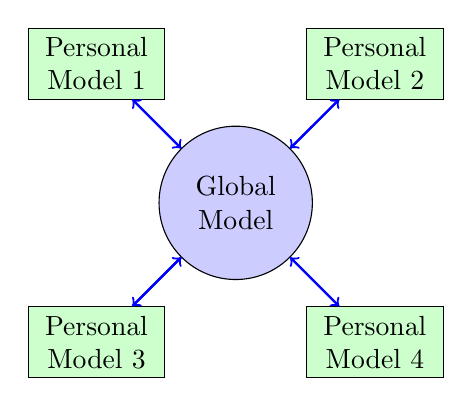
\begin{tikzpicture}[
    node distance=2.5cm,
    global/.style={circle, draw, fill=blue!20, text width=1.5cm, text centered},
    personal/.style={rectangle, draw, fill=green!20, text width=1.5cm, text centered},
    arrow/.style={->, thick, blue}
]
    % Global model
    \node[global] (global) {Global Model};
    
    % Personalized models
    \node[personal, above left of=global] (p1) {Personal Model 1};
    \node[personal, above right of=global] (p2) {Personal Model 2};
    \node[personal, below left of=global] (p3) {Personal Model 3};
    \node[personal, below right of=global] (p4) {Personal Model 4};
    
    % Bi-directional arrows
    \draw[arrow] (global) -- (p1);
    \draw[arrow] (p1) -- (global);
    \draw[arrow] (global) -- (p2);
    \draw[arrow] (p2) -- (global);
    \draw[arrow] (global) -- (p3);
    \draw[arrow] (p3) -- (global);
    \draw[arrow] (global) -- (p4);
    \draw[arrow] (p4) -- (global);
\end{tikzpicture}
\caption{Personalized Federated Learning Architecture}
\label{fig:personalized-fl}
\end{figure}

\begin{lstlisting}[language=python, caption=Personalized FL Algorithm]
class PersonalizedFederatedLearning:
    def __init__(self, personalization_strategy='meta_learning'):
        self.strategy = personalization_strategy
        self.global_model = None
        self.client_adaptations = {}
        
    def meta_learning_personalization(self, client_id, local_data):
        """Use meta-learning for rapid personalization"""
        # Model-Agnostic Meta-Learning (MAML) approach
        meta_model = self.global_model.copy()
        
        # Few-shot adaptation to local data
        personalized_model = self.maml_adaptation(
            meta_model=meta_model,
            adaptation_data=local_data,
            num_adaptation_steps=5,
            adaptation_lr=0.01
        )
        
        return personalized_model
        
    def clustered_personalization(self, clients_data):
        """Cluster clients and create specialized models"""
        # Cluster clients based on data characteristics
        client_clusters = self.cluster_clients_by_similarity(clients_data)
        
        cluster_models = {}
        for cluster_id, cluster_clients in client_clusters.items():
            # Train specialized model for each cluster
            cluster_model = self.train_cluster_specific_model(
                clients=cluster_clients,
                base_model=self.global_model
            )
            cluster_models[cluster_id] = cluster_model
            
        return cluster_models
        
    def federated_multi_task_learning(self, task_definitions):
        """Implement multi-task learning for related tasks"""
        shared_representation = self.learn_shared_representation(
            tasks=task_definitions,
            sharing_strategy='hard_parameter_sharing'
        )
        
        task_specific_heads = {}
        for task_id, task_def in task_definitions.items():
            task_head = self.create_task_specific_head(
                shared_repr=shared_representation,
                task_requirements=task_def
            )
            task_specific_heads[task_id] = task_head
            
        return shared_representation, task_specific_heads
\end{lstlisting}

\textbf{Federated Reinforcement Learning}
Extension of federated learning to reinforcement learning scenarios:

\begin{lstlisting}[language=python, caption=Federated Reinforcement Learning]
class FederatedReinforcementLearning:
    def __init__(self, environment_type, aggregation_method='policy_gradient'):
        self.environment_type = environment_type
        self.aggregation_method = aggregation_method
        self.global_policy = None
        
    def federated_policy_learning(self, client_experiences):
        """Learn global policy from distributed client experiences"""
        # Aggregate policy gradients from clients
        aggregated_gradients = self.aggregate_policy_gradients(
            client_experiences=client_experiences,
            weighting_scheme='experience_weighted'
        )
        
        # Update global policy
        self.global_policy = self.update_global_policy(
            current_policy=self.global_policy,
            aggregated_gradients=aggregated_gradients,
            learning_rate=0.001
        )
        
        return self.global_policy
        
    def distributed_value_function_learning(self, value_function_updates):
        """Learn shared value function across distributed agents"""
        # Federated learning for value function approximation
        global_value_function = self.federated_value_learning(
            local_updates=value_function_updates,
            aggregation_method='weighted_average',
            convergence_threshold=0.001
        )
        
        return global_value_function
        
    def multi_agent_coordination(self, coordination_objective):
        """Coordinate multiple agents through federated learning"""
        coordination_strategies = self.learn_coordination_strategies(
            objective=coordination_objective,
            communication_protocol='parameter_sharing',
            coordination_frequency='episodic'
        )
        
        return coordination_strategies
\end{lstlisting}

\subsubsection{Federated Learning on Edge and IoT}

\textbf{Ultra-Low Resource Federated Learning}
Algorithms designed for extremely resource-constrained devices:

\begin{lstlisting}[language=python, caption=Ultra-Low Resource FL]
class UltraLowResourceFL:
    def __init__(self, memory_limit_kb=64, compute_limit_mflops=10):
        self.memory_limit = memory_limit_kb * 1024  # bytes
        self.compute_limit = compute_limit_mflops * 1e6  # operations
        
    def microcontroller_friendly_training(self, model, local_data):
        """Training optimized for microcontrollers"""
        # Extreme quantization (1-bit or 2-bit)
        quantized_model = self.extreme_quantization(
            model=model,
            bits=2,
            quantization_scheme='dynamic'
        )
        
        # Gradient compression with error feedback
        compressed_gradients = self.ultra_compression(
            gradients=self.compute_gradients(quantized_model, local_data),
            compression_ratio=0.01,  # 99% compression
            error_feedback=True
        )
        
        return compressed_gradients
        
    def intermittent_computing_fl(self, power_profile):
        """FL for devices with intermittent power supply"""
        # Adaptive checkpoint frequency based on power availability
        checkpoint_strategy = self.adaptive_checkpointing(
            power_profile=power_profile,
            training_progress=self.get_training_state()
        )
        
        # Opportunistic training during power availability
        training_schedule = self.opportunistic_scheduling(
            power_windows=power_profile.available_windows,
            training_workload=self.estimate_training_cost()
        )
        
        return checkpoint_strategy, training_schedule
\end{lstlisting}

\subsection{Long-term Vision and Research Directions (3-10 years)}

Long-term research focuses on fundamental advances in federated learning theory, novel applications, and integration with emerging technologies.

\subsubsection{Neuromorphic Federated Learning}

Integration with neuromorphic computing architectures for ultra-efficient federated learning:

\begin{lstlisting}[language=python, caption=Neuromorphic FL Architecture]
class NeuromorphicFederatedLearning:
    def __init__(self, neuromorphic_hardware_type='loihi'):
        self.hardware_type = neuromorphic_hardware_type
        self.spike_encoding = SpikeEncodingManager()
        self.synaptic_plasticity = SynapticPlasticityEngine()
        
    def spike_based_federated_learning(self, spike_trains):
        """Implement FL using spike-based neural networks"""
        # Convert traditional neural networks to spiking networks
        spiking_network = self.convert_to_spiking_network(
            traditional_network=self.global_model,
            encoding_method='rate_coding'
        )
        
        # Federated learning with spike-timing-dependent plasticity
        federated_stdp = self.federated_spike_timing_plasticity(
            local_spike_trains=spike_trains,
            global_synaptic_weights=spiking_network.get_weights()
        )
        
        return federated_stdp
        
    def energy_efficient_inference(self, input_data):
        """Ultra-low power inference using neuromorphic principles"""
        # Event-driven computation
        spike_events = self.spike_encoding.encode_input(input_data)
        
        # Asynchronous processing
        inference_result = self.asynchronous_inference(
            spike_events=spike_events,
            network_state=self.get_network_state()
        )
        
        return inference_result
\end{lstlisting}

\subsubsection{Quantum Federated Learning}

Exploration of quantum computing applications in federated learning:

\begin{figure}[htbp]
\centering
\begin{tikzpicture}[
    node distance=2.5cm,
    quantum/.style={rectangle, draw, fill=purple!20, text width=2cm, text centered, minimum height=1cm},
    classical/.style={rectangle, draw, fill=orange!20, text width=2cm, text centered, minimum height=1cm},
    hybrid/.style={diamond, draw, fill=yellow!20, text width=1.5cm, text centered},
    arrow/.style={->, thick, purple}
]
    % Quantum-classical hybrid system
    \node[hybrid] (hybrid) {Quantum-Classical Interface};
    
    % Quantum components
    \node[quantum, above left of=hybrid] (q1) {Quantum Client 1};
    \node[quantum, above right of=hybrid] (q2) {Quantum Client 2};
    
    % Classical components
    \node[classical, below left of=hybrid] (c1) {Classical Client 1};
    \node[classical, below right of=hybrid] (c2) {Classical Client 2};
    
    % Connections
    \draw[arrow] (q1) -- (hybrid);
    \draw[arrow] (q2) -- (hybrid);
    \draw[arrow] (c1) -- (hybrid);
    \draw[arrow] (c2) -- (hybrid);
\end{tikzpicture}
\caption{Quantum-Classical Hybrid Federated Learning}
\label{fig:quantum-fl}
\end{figure}

\begin{lstlisting}[language=python, caption=Quantum Federated Learning]
class QuantumFederatedLearning:
    def __init__(self, quantum_backend='qiskit'):
        self.quantum_backend = quantum_backend
        self.quantum_circuits = {}
        self.variational_optimizer = VariationalQuantumOptimizer()
        
    def quantum_neural_network_fl(self, quantum_data):
        """Federated learning with quantum neural networks"""
        # Variational Quantum Eigensolver for optimization
        vqe_circuit = self.create_vqe_circuit(
            num_qubits=self.calculate_required_qubits(quantum_data),
            ansatz='hardware_efficient'
        )
        
        # Quantum federated averaging
        quantum_aggregation = self.quantum_parameter_aggregation(
            local_quantum_parameters=quantum_data.parameters,
            aggregation_method='quantum_averaging'
        )
        
        return quantum_aggregation
        
    def quantum_advantage_fl(self, classical_comparison):
        """Identify scenarios where quantum FL provides advantage"""
        quantum_advantage_metrics = {
            'exponential_speedup': self.analyze_exponential_speedup(),
            'quantum_entanglement_benefits': self.analyze_entanglement_advantages(),
            'quantum_parallelism': self.analyze_quantum_parallelism(),
            'fault_tolerance': self.analyze_quantum_error_correction()
        }
        
        return quantum_advantage_metrics
        
    def hybrid_quantum_classical_fl(self, hybrid_model):
        """Hybrid quantum-classical federated learning"""
        # Quantum layers for feature extraction
        quantum_features = self.quantum_feature_extraction(
            input_data=hybrid_model.classical_input,
            quantum_circuit=self.quantum_circuits['feature_extractor']
        )
        
        # Classical layers for final processing
        classical_output = self.classical_processing(
            quantum_features=quantum_features,
            classical_layers=hybrid_model.classical_layers
        )
        
        return classical_output
\end{lstlisting}

\subsubsection{Federated Learning for Emerging Applications}

\textbf{Federated Learning for Augmented/Virtual Reality}
Collaborative learning for AR/VR applications while preserving user privacy:

\begin{lstlisting}[language=python, caption=AR/VR Federated Learning]
class ARVRFederatedLearning:
    def __init__(self, reality_type='mixed_reality'):
        self.reality_type = reality_type
        self.spatial_understanding = SpatialUnderstandingEngine()
        self.user_behavior_analyzer = UserBehaviorAnalyzer()
        
    def collaborative_spatial_mapping(self, local_spatial_data):
        """Collaborative spatial understanding across AR devices"""
        # Privacy-preserving spatial feature extraction
        spatial_features = self.extract_privacy_preserving_spatial_features(
            spatial_data=local_spatial_data,
            privacy_method='differential_privacy'
        )
        
        # Federated learning for global spatial understanding
        global_spatial_model = self.federated_spatial_learning(
            local_features=spatial_features,
            aggregation_method='hierarchical_clustering'
        )
        
        return global_spatial_model
        
    def personalized_avatar_learning(self, user_interactions):
        """Learn personalized avatars through federated learning"""
        # Extract behavioral patterns while preserving privacy
        behavioral_features = self.extract_behavioral_features(
            interactions=user_interactions,
            anonymization_level='k_anonymity',
            k_value=10
        )
        
        # Federated learning for avatar personalization
        personalized_avatar_model = self.federated_avatar_learning(
            behavioral_features=behavioral_features,
            personalization_balance=0.7  # 70% personalization, 30% global
        )
        
        return personalized_avatar_model
\end{lstlisting}

\subsubsection{Theoretical Advances}

\textbf{Formal Privacy Guarantees}
Development of stronger theoretical foundations for privacy in federated learning:

\begin{lstlisting}[language=python, caption=Advanced Privacy Theory]
class AdvancedPrivacyTheory:
    def __init__(self):
        self.privacy_accountant = PrivacyAccountant()
        self.information_theory = InformationTheoreticPrivacy()
        
    def composition_theorems(self, privacy_mechanisms):
        """Advanced composition theorems for privacy guarantees"""
        # Optimal composition for multiple privacy mechanisms
        composed_privacy = self.optimal_composition(
            mechanisms=privacy_mechanisms,
            composition_type='advanced_composition'
        )
        
        # Concentrated differential privacy
        concentrated_dp = self.concentrated_differential_privacy(
            epsilon=composed_privacy.epsilon,
            delta=composed_privacy.delta,
            concentration_bounds=True
        )
        
        return concentrated_dp
        
    def information_theoretic_privacy(self, data_distribution):
        """Information-theoretic privacy measures"""
        # Mutual information privacy
        mi_privacy = self.mutual_information_privacy(
            data_distribution=data_distribution,
            privacy_mechanism=self.get_privacy_mechanism()
        )
        
        # Maximal leakage privacy
        max_leakage = self.maximal_leakage_privacy(
            prior_distribution=data_distribution.prior,
            posterior_distribution=data_distribution.posterior
        )
        
        return {
            'mutual_information_privacy': mi_privacy,
            'maximal_leakage': max_leakage
        }
\end{lstlisting}

\subsection{Integration with Emerging Technologies}

\subsubsection{Federated Learning and 6G Networks}

Preparation for 6G network integration with ultra-low latency and high reliability requirements:

\begin{lstlisting}[language=python, caption=6G Network Integration]
class SixGFederatedLearning:
    def __init__(self):
        self.network_slicing = NetworkSlicingManager()
        self.edge_intelligence = EdgeIntelligenceEngine()
        self.holographic_communication = HolographicCommEngine()
        
    def ultra_low_latency_fl(self, latency_requirement_ms=1):
        """Federated learning with ultra-low latency requirements"""
        # Network slicing for FL traffic
        fl_slice = self.network_slicing.create_fl_slice(
            latency_requirement=latency_requirement_ms,
            reliability_requirement=0.99999,  # 99.999% reliability
            bandwidth_requirement='1Gbps'
        )
        
        # Edge intelligence for local processing
        edge_processing = self.edge_intelligence.configure_edge_fl(
            processing_latency_budget=0.5,  # 0.5ms
            edge_computing_resources=fl_slice.allocated_resources
        )
        
        return fl_slice, edge_processing
        
    def holographic_fl_communication(self, holographic_data):
        """Federated learning for holographic communications"""
        # Holographic data compression for FL
        compressed_holo_data = self.holographic_communication.compress_holographic_model(
            holographic_model=holographic_data,
            compression_target='real_time_transmission'
        )
        
        return compressed_holo_data
\end{lstlisting}

\subsubsection{Metaverse and Web3 Integration}

Integration with decentralized technologies and virtual worlds:

\begin{lstlisting}[language=python, caption=Metaverse FL Integration]
class MetaverseFederatedLearning:
    def __init__(self):
        self.blockchain_integration = BlockchainFLIntegration()
        self.nft_models = NFTModelManager()
        self.dao_governance = DAOGovernanceEngine()
        
    def decentralized_model_marketplace(self):
        """Decentralized marketplace for federated learning models"""
        # NFT representation of trained models
        model_nfts = self.nft_models.create_model_nfts(
            trained_models=self.get_fl_models(),
            metadata_standard='ERC-721',
            provenance_tracking=True
        )
        
        # Smart contracts for model trading
        trading_contracts = self.blockchain_integration.deploy_model_trading_contracts(
            model_nfts=model_nfts,
            pricing_mechanism='bonding_curve',
            revenue_sharing=True
        )
        
        return model_nfts, trading_contracts
        
    def dao_governed_federated_learning(self, governance_token):
        """DAO-governed federated learning protocols"""
        # Governance proposals for FL parameters
        governance_proposals = self.dao_governance.create_fl_proposals(
            proposal_types=['privacy_budget', 'aggregation_method', 'client_selection'],
            governance_token=governance_token
        )
        
        return governance_proposals
\end{lstlisting}

\subsection{Research Collaboration and Open Science}

\subsubsection{Open Federated Learning Platforms}

Development of open-source platforms for collaborative research:

\begin{itemize}
    \item \textbf{Federated Learning Benchmarks}: Standardized benchmarks for comparing FL algorithms
    \item \textbf{Privacy-Preserving Datasets}: Synthetic datasets for FL research that preserve statistical properties
    \item \textbf{Reproducible Research Framework}: Tools for ensuring reproducibility in FL experiments
    \item \textbf{Cross-Platform Compatibility}: Standards for interoperability between different FL frameworks
\end{itemize}

\subsubsection{Industry-Academia Partnerships}

Fostering collaboration between research institutions and industry:

\begin{itemize}
    \item \textbf{Federated Learning Consortiums}: Multi-stakeholder consortiums for advancing FL research
    \item \textbf{Real-world Testbeds}: Deployment of FL systems in production environments for research
    \item \textbf{Privacy-Preserving Data Sharing}: Frameworks for sharing insights while protecting proprietary data
    \item \textbf{Standardization Efforts}: Contributing to international standards for federated learning
\end{itemize}

\subsection{Ethical and Societal Implications}

\subsubsection{Fairness and Bias Mitigation}

Advanced techniques for ensuring fairness in federated learning:

\begin{lstlisting}[language=python, caption=Fairness in Federated Learning]
class FairnessFederatedLearning:
    def __init__(self):
        self.fairness_metrics = FairnessMetricsEngine()
        self.bias_mitigation = BiasMitigationEngine()
        
    def fair_federated_aggregation(self, client_updates, fairness_constraints):
        """Aggregate client updates while ensuring fairness"""
        # Fairness-aware aggregation
        fair_aggregation = self.fairness_aware_aggregation(
            client_updates=client_updates,
            fairness_metric='equalized_odds',
            protected_attributes=fairness_constraints.protected_attributes
        )
        
        # Bias mitigation during aggregation
        debiased_model = self.bias_mitigation.debias_global_model(
            aggregated_model=fair_aggregation,
            bias_detection_method='statistical_parity'
        )
        
        return debiased_model
        
    def algorithmic_auditing_fl(self, fl_system):
        """Automated auditing of FL systems for bias and fairness"""
        audit_results = self.fairness_metrics.comprehensive_audit(
            fl_system=fl_system,
            audit_dimensions=['individual_fairness', 'group_fairness', 'counterfactual_fairness']
        )
        
        return audit_results
\end{lstlisting}

\subsection{Implementation Roadmap}

\begin{table}[H]
\centering
\caption{Future Work Implementation Timeline}
\label{tab:implementation-roadmap}
\resizebox{\textwidth}{!}{
\begin{tabular}{|l|l|l|l|}
\hline
\textbf{Timeline} & \textbf{Research Area} & \textbf{Key Deliverables} & \textbf{Expected Impact} \\
\hline
6 months & Performance Optimization & Advanced compression, client selection & 30\% efficiency gain \\
\hline
1 year & Security Enhancement & Quantum-resistant crypto & Future-proof security \\
\hline
2 years & Personalized FL & Meta-learning, clustering & Improved model relevance \\
\hline
3 years & Edge/IoT Integration & Ultra-low resource algorithms & IoT-scale deployment \\
\hline
5 years & Quantum FL & Hybrid quantum-classical & Quantum advantage \\
\hline
7 years & Neuromorphic FL & Spike-based learning & Ultra-low power \\
\hline
10 years & Metaverse Integration & Decentralized FL platforms & Web3 compatibility \\
\hline
\end{tabular}
}
\end{table}

\subsection{Competitive Analysis and Positioning}

To understand FLOPY-NET's position in the federated learning ecosystem, it's essential to compare it with existing solutions and identify areas for competitive advantage.

\subsubsection{Comparison with Existing FL Frameworks}

\begin{table}[H]
\centering
\caption{Comparison of Federated Learning Frameworks}
\label{tab:fl-framework-comparison}
\resizebox{\textwidth}{!}{
\begin{tabular}{@{}lcccccc@{}}
\toprule
\textbf{Framework} & \textbf{SDN Integration} & \textbf{Policy Engine} & \textbf{Network Simulation} & \textbf{Real-time Monitoring} & \textbf{Container Orchestration} & \textbf{Open Source} \\
\midrule
FLOPY-NET & \checkmark & \checkmark & \checkmark (GNS3) & \checkmark & \checkmark & \checkmark \\
NVIDIA Flare & \texttimes & Partial & \texttimes & \checkmark & \checkmark & \checkmark \\
TensorFlow Federated & \texttimes & \texttimes & \texttimes & Partial & \texttimes & \checkmark \\
FedML & \texttimes & \texttimes & \texttimes & \checkmark & Partial & \checkmark \\
OpenFL & \texttimes & Basic & \texttimes & \checkmark & \checkmark & \checkmark \\
Flower & \texttimes & \texttimes & \texttimes & Basic & Partial & \checkmark \\
PySyft & \texttimes & Privacy-focused & \texttimes & Basic & \texttimes & \checkmark \\
\bottomrule
\end{tabular}
}
\end{table}

\subsubsection{Competitive Advantages}

\textbf{Network-Centric Approach}
\begin{itemize}
    \item \textbf{SDN Integration}: FLOPY-NET is unique in providing native SDN controller integration for network optimization
    \item \textbf{GNS3 Simulation}: Real network topology simulation capabilities not found in other FL frameworks
    \item \textbf{Network-Aware Policies}: Dynamic network condition response through policy engine
\end{itemize}

\textbf{Observatory Architecture}
\begin{itemize}
    \item \textbf{Comprehensive Monitoring}: Multi-layer observability from network to application level
    \item \textbf{Real-time Analytics}: Live dashboard with cross-component metrics correlation
    \item \textbf{Policy-Driven Operations}: Centralized governance through flexible policy engine
\end{itemize}

\subsubsection{Detailed Framework Analysis}

\textbf{NVIDIA Flare Comparison}

NVIDIA Flare is currently the most mature enterprise FL platform. Key differences:

\begin{table}[H]
\centering
\caption{FLOPY-NET vs NVIDIA Flare}
\label{tab:flopynet-vs-nvidia-flare}
\begin{tabularx}{\textwidth}{@{}lXX@{}}
\toprule
\textbf{Aspect} & \textbf{FLOPY-NET} & \textbf{NVIDIA Flare} \\
\midrule
Network Focus & SDN-native with GNS3 simulation & Application-layer only \\
Policy Management & Centralized policy engine with network integration & Configuration-based governance \\
Monitoring & Multi-layer observatory with real-time dashboard & Admin console with job monitoring \\
Deployment & Docker Compose with container orchestration & Kubernetes-native deployment \\
Use Case & Research \& network optimization & Enterprise production deployments \\
Learning Curve & Moderate (research-oriented) & Steep (enterprise-focused) \\
\bottomrule
\end{tabularx}
\end{table}

\textbf{TensorFlow Federated Comparison}

TensorFlow Federated focuses on algorithmic research:

\begin{table}[H]
\centering
\caption{FLOPY-NET vs TensorFlow Federated}
\label{tab:flopynet-vs-tff}
\begin{tabularx}{\textwidth}{@{}lXX@{}}
\toprule
\textbf{Aspect} & \textbf{FLOPY-NET} & \textbf{TensorFlow Federated} \\
\midrule
Scope & End-to-end FL platform & Algorithm development framework \\
Deployment & Production-ready containers & Simulation environment \\
Network Modeling & Real network simulation & Abstract communication \\
Monitoring & Comprehensive system monitoring & Research metrics only \\
Scalability & Container-based horizontal scaling & Single-machine simulation \\
Integration & Multi-service architecture & TensorFlow ecosystem only \\
\bottomrule
\end{tabularx}
\end{table}

\subsubsection{Future Competitive Positioning}

\textbf{Research Community Advantages}
\begin{itemize}
    \item \textbf{Network Research}: Unique platform for network-aware FL research
    \item \textbf{Policy Research}: Flexible policy engine for governance research
    \item \textbf{System Research}: End-to-end platform for systems research
\end{itemize}

\textbf{Industry Applications}
\begin{itemize}
    \item \textbf{Telecommunications}: Network optimization for 5G/6G FL deployments
    \item \textbf{Edge Computing}: Network-aware edge FL orchestration
    \item \textbf{IoT Ecosystems}: Policy-driven IoT FL coordination
\end{itemize}

\subsection{Conclusion}

The future of federated learning lies in addressing fundamental challenges while exploring new frontiers. The FLOPY-NET framework is positioned to evolve with these advances, providing a robust foundation for next-generation federated learning applications. The research directions outlined in this section will ensure that the framework remains at the forefront of federated learning technology, enabling new applications and addressing emerging challenges in privacy-preserving distributed machine learning.

Key areas of focus include:
\begin{itemize}
    \item Advancing the theoretical foundations of federated learning
    \item Developing practical solutions for resource-constrained environments
    \item Ensuring fairness, privacy, and security in large-scale deployments
    \item Exploring integration with emerging technologies
    \item Fostering open science and collaborative research
\end{itemize}

This comprehensive roadmap provides a clear path forward for the continued development and evolution of the FLOPY-NET framework, ensuring its relevance and impact in the rapidly evolving landscape of federated learning and distributed machine learning.

\subsection{Competitive Analysis}

FLOPY-NET provides unique capabilities compared to existing federated learning platforms. This section analyzes the architectural differences and positioning relative to major platforms like NVIDIA Flare, IBM FL, and PySyft.

\subsubsection{Platform Comparison}

\begin{table}[H]
\centering
\caption{Federated Learning Platform Comparison}
\label{tab:platform-comparison}
\resizebox{\textwidth}{!}{%
\begin{tabular}{@{}lllll@{}}
\toprule
\textbf{Feature} & \textbf{FLOPY-NET} & \textbf{NVIDIA Flare} & \textbf{IBM FL} & \textbf{PySyft} \\
\midrule
\textbf{Core Focus} & Network-aware FL + SDN & Framework-agnostic FL & Enterprise FL & Privacy-preserving FL \\
\textbf{Architecture} & Microservices + Docker & Client-Server + SDK & Modular components & Differential privacy \\
\textbf{Network Integration} & Native SDN/GNS3 & Limited & No & No \\
\textbf{Policy Engine} & Central governance & Security plugins & Basic rules & Privacy policies \\
\textbf{Real-time Monitoring} & Comprehensive dashboard & TensorBoard integration & Basic monitoring & Limited \\
\textbf{Container Support} & Native Docker deployment & Manual setup & Kubernetes support & Docker available \\
\textbf{Network Simulation} & GNS3 + Ryu controller & No & No & No \\
\textbf{Multi-framework} & PyTorch/TensorFlow & PyTorch/TensorFlow/JAX & Multiple & PyTorch \\
\textbf{Deployment Scale} & Research + Production & Production-focused & Enterprise-scale & Research-focused \\
\textbf{License} & Open Source & Apache 2.0 & Apache 2.0 & Apache 2.0 \\
\bottomrule
\end{tabular}%
}
\end{table}

\subsubsection{Unique Value Proposition}

FLOPY-NET's distinguishing characteristics include:

\begin{itemize}
    \item \textbf{Network-Centric Design}: Unlike other platforms that treat the network as transparent, FLOPY-NET makes network conditions a first-class citizen in FL research
    \item \textbf{Policy-Driven Architecture}: Central policy engine governs all system interactions, ensuring compliance and security
    \item \textbf{Research-Oriented Network Simulation}: Integration with GNS3 and SDN controllers enables realistic network condition simulation
    \item \textbf{Container-Native Deployment}: Purpose-built for containerized environments with Docker Compose orchestration
    \item \textbf{Real-time Observability}: Comprehensive metrics collection and dashboard provide unprecedented system visibility
\end{itemize}

\subsubsection{Technical Architecture Comparison}

\begin{table}[H]
\centering
\caption{Technical Architecture Comparison}
\label{tab:architecture-comparison}
\begin{tabularx}{\textwidth}{@{}lXX@{}}
\toprule
\textbf{Component} & \textbf{FLOPY-NET} & \textbf{NVIDIA Flare} \\
\midrule
\textbf{Server Architecture} & GRPC + FastAPI + HTTP REST APIs + Custom protocols & GRPC + Custom protocols \\
\textbf{Client Communication} & HTTP + WebSocket & GRPC streaming \\
\textbf{Configuration Management} & Policies + JSON + Environment variables & YAML + Job definitions \\
\textbf{Network Layer} & Ryu SDN controller + GNS3 & Standard networking \\
\textbf{Monitoring} & Real-time dashboard + metrics & TensorBoard + logs \\
\textbf{Policy Management} & SQLite + REST API & Event-based security plugins \\
\textbf{Data Storage} & SQLite + JSON metrics & Job-specific storage \\
\textbf{Deployment} & Docker Compose + static IPs & Kubernetes + dynamic \\
\bottomrule
\end{tabularx}
\end{table}

\subsubsection{Use Case Positioning}

Based on the architectural analysis, FLOPY-NET is positioned for:

\begin{itemize}
    \item \textbf{Network Research}: Studies on the impact of network conditions on FL performance
    \item \textbf{Policy Compliance}: Scenarios requiring strict governance and audit trails
    \item \textbf{Educational Environments}: Teaching FL concepts with visual network simulation
    \item \textbf{Prototype Development}: Rapid development and testing of FL algorithms
    \item \textbf{Multi-domain Experiments}: Cross-organizational FL with policy enforcement
\end{itemize}

While NVIDIA Flare excels in production deployments and enterprise scale, FLOPY-NET provides unique capabilities for network-aware federated learning research and education.

\subsection{Conclusion}

The future work outlined in this section represents a comprehensive roadmap for advancing FLOPY-NET's capabilities across multiple dimensions. From short-term algorithmic improvements to long-term integration with emerging technologies like quantum computing and 6G networks, these research directions will ensure FLOPY-NET remains at the forefront of federated learning research infrastructure.

The emphasis on privacy-preserving techniques, scalability improvements, and real-world deployment considerations reflects the evolving needs of the federated learning community. By pursuing these research directions systematically, FLOPY-NET will continue to serve as a valuable platform for both fundamental research and practical applications in distributed machine learning.
